\documentclass[../thesis/thesis.tex]{subfiles}
\begin{document}
\chapter{Literature Review}
\label{chap:litreview}

Within this chapter we consider the broad variety of sensing systems available, and how well different types of sensors meet our sensing criteria. It can be difficult to approach the broad variety of sensor types in the field, so a structure must be developed through which to evaluate them. Teixeira, Dublon and Savvides~\cite{teixeira2010survey} propose a 5-element human-sensing criteria which provides a structure through which we may define the broad quantitative requirements of different sensors.

These quantitative requirements can be used to exclude sensing options that clearly cannot meet the requirements before the more specific qualitative accessibility criteria will be considered for those remaining sensors. 

The quantitative criteria elements are;
\begin{enumerate}
 \item \emph{Presence}: Is there any occupant present in the sensed area?
 \item \emph{Count}: How many occupants are there in the sensed area?
 \item \emph{Location}: Where are the occupants in the sensed area?
 \item \emph{Track}: Where do the occupants move in the sensed area? (local identification)
 \item \emph{Identity}: Who are the occupants in the sensed area? (global identification)
\end{enumerate}

At a fundamental level, this research project requires a sensor system that provides both Presence and Count information. To assist with the reduction of privacy concerns, excluding systems that permit Identity information will generally result in a less invasive system also. The presence of Location or Track information are irrelevant to our project's goals, but overall, minimizing these elements should in most cases help to maximize the energy efficiency of the system also.

Teixeira, Dublon and Savvides~\cite{teixeira2010survey} also propose an occupancy sensor taxonomy (see \Fref{fig:litreview:taxonomy}), which categorizes different sensing systems in terms of what information they use as a proxy for human-sensing. We use this taxonomy here as a structure through which we group and discuss different sensor types.

\begin{figure}
\centering
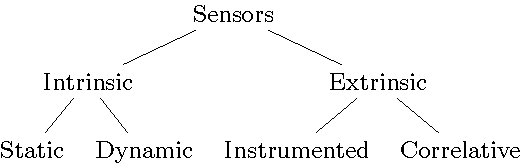
\includegraphics{../diagrams/category-tree.pdf}
\caption{Occupancy sensor taxonomy proposed by Teixeira, Dublon and Savvides~\cite{teixeira2010survey}}
\label{fig:litreview:taxonomy}
\end{figure}

\section{Intrinsic traits}
\label{subsec:litreview:sensors:intrinsic}

Intrinsic traits are those which can be sensed that are a direct property of being a human occupant. Intrinsic traits are particularly useful, as in many instances they are guaranteed to be present if an occupant is present. However, they do have varying degrees of detectability and differentiation between occupants. Two main subcategories of these sensor types are static and dynamic traits.

\subsection{Static traits}
\label{subsubsec:litreview:sensors:intrinsic:static}
Static traits are physiologically derived, and are present with most (living) occupants. One key static trait that can be used for occupant sensing is that of thermal emissions. All human occupants emit distinctive thermal radiation in both resting and active states. The heat signatures of these emissions could potentially be measured with some apparatus, counted, and used to provide Presence and Count information to a sensor system, without providing Identity information.

Beltran, Erickson and Cerpa~\cite{beltran2013thermosense} propose ThermoSense, a system that uses a type of thermal sensor known as a \iar. This sensor is much like a camera, in that it has a field of view which is divided into ``pixels''; in this case an $8\times8$ grid of detected temperatures. This sensor is mounted on an embedded device on the ceiling, along with a \pir for basic motion detection, and uses machine learning algorithms to detect human heat signatures within the raw thermal and motion data it collects. ThermoSense measures accuracy with Root Mean Squared Error (RMSE), an average of the absolute value that their prediction deviated from the true result. They achieve an RMSE of 0.35 occupants, which they indicate is sufficient for accurate occupancy detection.

Another static trait is that of \cdi emissions, which, like thermal emissions, are emitted by human occupants in both resting and active states. By measuring the build-up of \cdi within a given area, one can use a variety of mathematical models of human \cdi production to determine the likely number of occupants present. Hailemariam \etal~\cite{hailemariam2011real} trialled this as part of a sensor fusion within the context of an office environment, achieving a $\approx94\%$ accuracy. Such a sensing system could provide both the Presence and Count information, and exclude the Identity information as required. However, \cdi based detection methods have serious drawbacks, discussed by Fisk, Faulkner and Sullivan~\cite{fisk2006accuracy}: The \cdi feedback mechanism is slow, taking hours of continuous occupancy to correctly identify the presence of people. In a residential environment, occupants are more likely to be moving between rooms than an office, so the system may have a more difficult time detecting in that situation. Similarly, such systems can be interfered with by other elements that control the \cdi build-up in a space, like air conditioners and open windows. This is also much more of a concern in a residential environment compared to the studied office space, as the average residence can have numerous such confounding factors that cannot easily be controlled for.

Occupant identification can also be achieved through the use of video or still-image cameras and advanced image processing algorithms. Video can be used in occupancy detection in several different ways, achieving different levels of accuracy and requiring different configurations. The first use of video, POEM, proposed by Erickson, Achleitner and Cerpa~\cite{erickson2013poem} is the use of video as a ``optical turnstile'': The video system detects potential occupants and the direction they are moving in at each entrance and exit to an area, and uses that information to extrapolate the number of occupants within the turnstiled area. They report the system achieves up to a 94\% accuracy. However, the main issue with such a system applied to a residential environment is the system assumes that there will be wide enough ``turnstile areas'', corridors of a fairly large area that connect different sections of a building, to use as detection zones. While such corridors exist in office environments, they are less likely to exist in residential ones.

Another video-based sensor system is proposed by Serrano-Cuerda \etal~\cite{serrano2013efficient}, that uses ceiling-based cameras and advanced image processing algorithms to count the number of people in the captured area. They measure accuracy using an F-score, which takes into account both false-positive and false-negative results, and is reported as 0.967, which is highly accurate. Such a system could be successfully applied to the residential environment, as both it and the ``optical turnstile'' model provide Presence and Count information. However, these systems also allow Identity to be determined, and thus are perceived as privacy-invasive.

\subsection{Dynamic traits}
\label{subsubsec:litreview:sensors:intrinsic:dynamic}
Dynamic traits are usually products of human occupant activity, and thus can generally only be detected when a human occupant is physically active or in motion.

Ultrasonic systems, such as Doorjamb proposed by Hnat \etal~\cite{hnat2012doorjamb}, use clusters of such sensors above door-frames to detect the height and direction of potential occupants travelling between rooms. This acts as a turnstile based system, much like POEM~\cite{erickson2013poem}, but augments this with an understanding of the model of the building to correct for invalid and impossible movements brought about from sensing errors. This system provides an overall room-level tracking accuracy of 90\%, however to achieve this accuracy, potential occupants are intended to be tracked using their heights, which has privacy implications. The system can also suffer from problems with error propagation, as there are possibilities of ``phantom'' occupants entering a room due to sensing errors.

Solely \pir based systems, like those used by Hailemariam \etal~\cite{hailemariam2011real}, involve the motion of the sensor being averaged over several different time intervals, and fed into a decision tree classifier. This \pir system alone produced a $\approx98\%$ accuracy. However, such a system, due to only motion detection capabilities, can only provide Presence information, and is unable to provide Count information, or detect motionless occupants.

\section{Extrinsic traits}
\label{subsec:litreview:sensors:extrinsic}
Extrinsic traits are those which are actually other environmental changes that are caused by or correlated with human occupant presence. These traits generally present a less accurate picture, or require the sensed occupants to be in some way ``tagged'', but they are generally also easier to sense themselves. The sensors in this category have been divided into two subcategories.

\subsection{Instrumented traits}
\label{subsubsec:litreview:sensors:extrinsic:instrumented}
One extrinsic trait category is instrumented approaches; these require that detectable occupants carry with them some device that is detected as a proxy for the occupant themselves.

The most obvious of these approaches is a specially designed device. Li \etal~\cite{li2012measuring} used RFID tags and several antennas as a triangulation and tracking mechanism to pinpoint tag-carrying occupants to a specific HVAC thermal zone. For stationary occupants, there was a detection accuracy of $\approx88\%$, and for occupants who were mobile, the accuracy was $\approx62\%$. Such a system could be re-purposed for the residence, however it requires occupants to be constantly carrying their tags, which is less likely in such an environment. Additionally, the accuracy for this system is not necessarily high enough for a residential environment, where much smaller rooms are used.

To make extrinsic detection more reliable, Li, Calis and Becerik-Gerber~\cite{kleiminger2013inferring} leverage a common consumer device; WiFi enabled smart phones. They propose the \textit{homeset} algorithm, which uses the phones to scan the visible WiFi networks, and from that information estimate if the occupants are present or absent in their home by ``triangulating'' their position from the visible WiFi networks. This solution does not provide the fine-grained Presence data that we need, as it is only able to triangulate the phone's position to a large error margin with the wireless network detection information.

Balaji \etal~\cite{balaji2013sentinel} also leverage smart phones to determine occupancy, but in a more broad enterprise environment: Wireless device association logs are analysed to determine which access points in a building a given occupant is connected to. If this access point falls within the radio range of their designated ``personal space'', they are considered to be occupying that personal space. This technique cannot be applied to a residential environment, as there are usually not multiple wireless hotspots present.

Finally, Gupta, Intille and Larson~\cite{gupta2009adding} use specifically the GPS functions of the smartphone to perform optimisation on heating and cooling systems by calculating the ``travel-to-home'' time of occupants at all times and ensuring at every distance the house is minimally heated such that if the potential occupant were to travel home, the house would be at the correct temperature when they arrived. While this system does achieve similar potential air-conditioning energy savings, it is not room-level modular, and also presupposes an occupant whose primary energy costs are from incorrect heating when away from home, which isn't necessarily the case for the elderly or disabled demographics considered in this dissertation.

\subsection{Correlative traits}
\label{subsubsec:litreview:sensors:extrinsic:correlative}
The second of our discussed subcategories are correlative approaches. These approaches analyse data that is correlated with human occupant activity, but does not require a specific device to be present on each occupant that is tracked with the system.

The primary approach in this area is work done by Kleiminger \etal~\cite{kleiminger2013occupancy}, which attempts to measure electricity consumption and use such data to determine Presence. Electricity data was measured at two different levels of granularity; the whole house level with a smart meter, and the consumption of specific appliances through smart plugs. This data was then processed by a variety of classifiers to achieve a classification accuracy of more than 80\%. Such a system presents a low-cost solution to occupancy, however it is not sufficiently granular in either the detection of multiple occupants, or the detection of occupants in a specific room. Additionally, it may be too invasive, due to the number of sensors and sensor plugs involved.

\section{Analysis}
\label{sec:litreview:sensors:analysis}

\begin{table}[h]
\begin{threeparttable}
\begin{tabularx}{\textwidth}{|l|l|l||l||l|l|}
\cline{2-6}
\multicolumn{1}{r|}{}		    	& \multicolumn{2}{c||}{Requires} & Excludes & \multicolumn{2}{c|}{Irrelevant} \\
\cline{2-6}
\multicolumn{1}{r|}{}		    	& \csbox{Presence} & \csbox{Count} & \csbox{Identity} & \csbox{Location} & \csbox{Track} \\
\cline{1-6}

\underline{Intrinsic} 			& & & & & \\
\hspace{3mm}\textit{Static} 		& & & & & \\
\hspace{8mm}Thermal 			& \cmark & \cmark & \cmark & \cmark &  \\
\hspace{8mm}\cdi			& \cmark & \cmark & \cmark &  &  \\
\hspace{8mm}Video			& \cmark & \cmark & \xmark & \cmark & \cmark \\

\hspace{3mm}\textit{Dynamic} 		& & & & & \\
\hspace{8mm}Ultrasonic	 		& \cmark & \cmark & \xmark & & \cmark \\
\hspace{8mm}PIR		 		& \cmark & \xmark & \cmark &  &  \\

					& & & & & \\

\underline{Extrinsic}			& & & & & \\
\hspace{3mm}\textit{Instrumented} 	& & & & & \\
\hspace{8mm}RFID 			& \cmark\ssup & \cmark & \cmark & \cmark & \\
\hspace{8mm}WiFi assoc.\tsup		& \cmark\ssup & \cmark & \xmark & \cmark & \\
\hspace{8mm}WiFi triang.\tsup		& \cmark\ssup & \cmark & \xmark & & \\
\hspace{8mm}GPS\tsup			& \cmark\ssup & \xmark & \cmark & \cmark & \\

\hspace{3mm}\textit{Correlative} 	& & & & & \\
\hspace{8mm}Electricity 		& \cmark\ssup & \xmark & \cmark & & \\

\cline{1-6}
\end{tabularx}
\begin{tablenotes}
\item \ssup  Doesn't provide data at required level of accuracy for home use.
\item \tsup  Uses smartphone as detector.
\end{tablenotes}
\end{threeparttable}
\caption{Comparison of information provided by different sensors types discussed with reference to the project's requirements}
\label{tab:litreview:taxonomycomp}
\end{table}

From these various sensor options, there are a few candidates that provide the necessary quantitative criteria (Presence and Count); these are thermal, \cdi, Video, Ultrasonic, RFID, WiFi association and WiFi triangulation based methods. All sensing options are compared in \Fref{tab:litreview:taxonomycomp}.

In the context of our four qualitative accessibility criteria, \cdi sensing has several reliability drawbacks, the predominant ones being a large lag time to receive accurate occupancy information and interference from a variety of air conditioning sources which can modify the \cdi concentration in the room in unexpected ways.

Video-based sensing methods suffer from invasiveness concerns, as they by design must have a constant video feed of all detected areas.

Ultrasonic methods suffer from reliability concerns when a user falls outside the prescribed height bounds of average humans. The detection accuracy of wheelchair bound occupants, a potential demographic of our proposed sensing system, are not discussed in the Doorjamb paper. The paper indicates various complications such as hats or carrying items may affect the detection, which suggests that a wheelchair may do the same. Ultrasonic methods also provide weak Identity information through height detection.

RFID sensing also has several drawbacks; it is a difficult value proposition to get residential occupants to carry RFID tags with them continuously. Another drawback is that the triangulation methods discussed are too unreliable to place occupants in specific rooms in many cases, and may suffer from read range issues depending on the specific RFID technologies used.

WiFi association is not granular enough for residential use, as the original enterprise use case presupposes a much larger area, as well as multiple wireless access points, neither of which a typical residential environment has.

WiFi triangulation is a good candidate for residential use, as there are most likely neighbouring wireless networks that can be used as virtual landmarks. However, it suffers from the same granularity problems as WiFi association, as these signals are not specific enough to pinpoint an occupant to a specific room.

For approaches presupposing smartphones being present on each occupant, it similarly difficult to ensure that occupants are carrying their smartphones with them at all times in a residential environment, as with RFID tags.  Another issue with smart phones is that they can represent an expense that the target markets of the elderly and the disabled may not be able to afford, as opposed to a dumb mobile or landline phone.

Finally, we have thermal sensing. It provides both Presence and Count information, as it uses occupants' thermal signatures to determine the presence of people in a room. It does not however provide Identity information, as thermal signatures are not sufficiently unique with the technologies used to distinguished between occupants. Such a sensor system is presented as low-cost and energy efficient within ThermoSense~\cite{beltran2013thermosense}. The system non-invasive by design and can reliably detect occupants with a low Root Mean Squared Error. For our specific accessibility criteria, thermal sensing appears to be the most suitable option.

\section{Research Gap}
ThermoSense's ``Grid-EYE''-based sensing system has the potential to meet our goals of low cost, non-invasiveness, reliability and energy efficiency. However, their approach has room for improvement. The TMote Sky, the embedded controller for the ThermoSense design, is expensive (estimated to be \$100+), outdated (released in 2006) and does not appear available for sale in Australia (manufacturer's website is no longer available). Additionally, the Grid-EYE sensor is also not available to purchase within Australia, nor to order into Australia from other countries.

Furthermore, the robustness of the ThermoSense approach is currently unexplored. Is their approach applicable to a similar sensor in a slightly different environment? Does their approach generalize well? There still exists many unknown quantities that are worthwhile to explore.

We believe there is a clear gap within the Australian market for an occupancy sensor that meets these goals. Additionally, there exist important unanswered questions regarding the reliability and robustness of the approach ThermoSense used. Finally, as the Grid-EYE cannot be used, an investigation into how well a substitute sensor can meet replicate ThermoSense's results will be necessary.

\ifcsdef{mainfile}{}{\bibliography{../references/primary}}
\end{document}